% Source: Graph_ML/Graph_AE/graph_autoencoders_tutorial.tex
\begin{notechapter}
% ---- chapter-local definitions ----
\forgetcs\hadamard\newcommand{\hadamard}{\odot}
% -----------------------------------
\chapter{Graph Autoencoders}\label{ch:graph-autoencoders}
\chaptersubtitle{SDNE, GAE and VGAE}

\begin{chapterintro}
An autoencoder compresses its input into a low-dimensional code and reconstructs the input from it. Applied to a graph, the natural input of a node is its row of the adjacency matrix, and the code is the node's embedding. This chapter explains why the plain reconstruction loss fails on sparse graphs and how the structural deep network embedding (SDNE) of Wang, Cui and Zhu (\emph{Structural Deep Network Embedding}, 2016) repairs it with two terms: a weighted reconstruction loss that preserves second-order proximity, and a Laplacian penalty that preserves first-order proximity. It then presents the graph autoencoders of Kipf and Welling (\emph{Variational Graph Auto-Encoders}, 2016), whose encoder is a GCN and whose decoder is an inner product. You will learn
\begin{itemize}[nosep]
  \item the SDNE loss $\mathcal L_{2^{nd}} + \alpha\mathcal L_{1^{st}} + \lambda\mathcal L_{reg}$, what each term does, and how to compute it on small examples;
  \item why the first-order term is the Laplacian quadratic form $2\tr(Y^\top LY)$, and why the two terms are complementary;
  \item what an encoder that reads adjacency rows can and cannot distinguish;
  \item GAE and VGAE, and how they relate to SDNE and to the shallow embeddings of \cref{ch:shallow-embeddings}.
\end{itemize}
\prerequisites{autoencoders and the evidence lower bound (variational autoencoders); \cref{ch:graph-laplacians} (Laplacian quadratic form) and \cref{ch:shallow-embeddings} (first- and second-order proximity); the GCN layer of \cref{ch:dft-to-gnn}.}
\end{chapterintro}

\section{Introduction}

Graph autoencoders extend the classical autoencoder framework to handle graph-structured data. While the encoder-decoder architecture remains conceptually similar, the design of appropriate loss functions requires careful consideration of the unique properties of graph structures.

\subsection{The Autoencoder Framework}

A classical autoencoder consists of:
\begin{itemize}
    \item \textbf{Encoder}: $f: \R^n \to \R^d$ where $d \ll n$ (dimensionality reduction)
    \item \textbf{Decoder}: $g: \R^d \to \R^n$ (reconstruction)
    \item \textbf{Loss function}: Typically $\mathcal{L} = \norm{x - g(f(x))}^2$ (reconstruction error)
\end{itemize}

The goal is to learn a compressed representation that preserves the essential information in the input.

\subsection{Challenges with Graph Structures}

When applying autoencoders to graphs, several critical issues arise:

\begin{enumerate}
    \item \textbf{Sparsity}: Adjacency matrices are extremely sparse (most entries are 0)
    \item \textbf{Asymmetric information}: Edge presence ($A_{ij} = 1$) is informative, but edge absence ($A_{ij} = 0$) does not necessarily indicate dissimilarity
    \item \textbf{Imbalanced learning}: The model naturally tends to predict 0 everywhere to minimize standard reconstruction error
\end{enumerate}

\begin{keyidea}
Standard reconstruction loss treats all errors equally. For sparse graphs, this leads to trivial solutions where the model learns to output all zeros.
\end{keyidea}

We use the two notions of proximity of \cref{ch:shallow-embeddings}: nodes have high \emph{first-order} proximity when they are joined by an edge, and high \emph{second-order} proximity when their neighbourhoods (rows of $\bm A$) are similar. SDNE has one loss term for each.

\section{Loss Function 1: Second-Order Proximity}

\subsection{Mathematical Formulation}

The second-order proximity loss is defined as:
\begin{equation}
\mathcal{L}_{2^{nd}} = \sum_{i} \norm{(\tilde{\bm{A}}_i - \bm{A}_i) \hadamard \bm{B}_i}^2
\label{graph-autoencoders:eq:l2_loss}
\end{equation}

where:
\begin{itemize}
    \item $\bm{A}_i \in \R^n$: The $i$-th row of the adjacency matrix (neighborhood of node $i$)
    \item $\tilde{\bm{A}}_i \in \R^n$: The $i$-th row of the reconstructed adjacency matrix
    \item $\bm{B}_i \in \R^n$: Weight vector with entries:
    \begin{equation}
    B_{ij} = \begin{cases}
    \beta & \text{if } A_{ij} = 1 \\
    1 & \text{if } A_{ij} = 0
    \end{cases}
    \end{equation}
    \item $\hadamard$: Hadamard (element-wise) product
    \item $\beta > 1$: Hyperparameter controlling the penalty for edge reconstruction errors (typically $\beta \in [5, 10]$)
\end{itemize}

\subsection{Intuition Behind the Weighting}

The key innovation is the weight vector $\bm{B}_i$. By setting $B_{ij} = \beta$ when an edge exists, we penalize errors on existing edges much more heavily than errors on non-edges.

\begin{intuition}[Why this works]
\begin{itemize}
    \item If the model predicts $\tilde{A}_{ij} = 0.1$ when $A_{ij} = 1$, the term is $(0.9\,\beta)^2 = 0.81\,\beta^2$, large. (The weight multiplies the error before squaring, so an edge counts $\beta^2$ times as much as a non-edge.)
    \item If the model predicts $\tilde{A}_{ij} = 0.1$ when $A_{ij} = 0$, the term is $(0.1)^2 = 0.01$, small
    \item This forces the model to focus on correctly reconstructing existing edges
\end{itemize}
\end{intuition}

\subsection{Detailed Example: Computing $\mathcal{L}_{2^{nd}}$}

\begin{example}[Second-Order Loss Calculation]
Consider a 5-node graph where node $i$ has the following adjacency vector:
\[
\bm{A}_i = [0, 1, 1, 0, 1]
\]
Node $i$ is connected to nodes 2, 3, and 5.

The autoencoder produces a reconstruction:
\[
\tilde{\bm{A}}_i = [0.1, 0.8, 0.9, 0.05, 0.7]
\]

With $\beta = 5$, the weight vector is:
\[
\bm{B}_i = [1, 5, 5, 1, 5]
\]

\textbf{Step 1}: Compute the reconstruction error:
\[
\bm{A}_i - \tilde{\bm{A}}_i = [-0.1, 0.2, 0.1, -0.05, 0.3]
\]

\textbf{Step 2}: Apply element-wise weighting:
\[
(\bm{A}_i - \tilde{\bm{A}}_i) \hadamard \bm{B}_i = [-0.1, 1.0, 0.5, -0.05, 1.5]
\]

\textbf{Step 3}: Compute squared norm:
\begin{align*}
\mathcal{L}_{2^{nd}}(i) &= \norm{[-0.1, 1.0, 0.5, -0.05, 1.5]}^2 \\
&= (-0.1)^2 + (1.0)^2 + (0.5)^2 + (-0.05)^2 + (1.5)^2 \\
&= 0.01 + 1.0 + 0.25 + 0.0025 + 2.25 \\
&= 3.5125
\end{align*}

\textbf{Comparison without weighting} ($\beta = 1$):
\begin{align*}
\mathcal{L}_{2^{nd}-{unweighted}}(i) &= (-0.1)^2 + (0.2)^2 + (0.1)^2 + (-0.05)^2 + (0.3)^2 \\
&= 0.01 + 0.04 + 0.01 + 0.0025 + 0.09 = 0.1525
\end{align*}
The weighted version is about $23$ times larger. This demonstrates how the weighting scheme dramatically increases the penalty for errors on existing edges.
\end{example}

\subsection{Why "Second-Order"?}

The loss function preserves second-order proximity because:

\begin{intuition}[Second-order proximity]
If nodes $i$ and $j$ have similar adjacency vectors ($\bm{A}_i \approx \bm{A}_j$), minimizing $\mathcal{L}_{2^{nd}}$ tends to give them similar embeddings.
The encoder maps adjacency vectors to embeddings. If $\bm{A}_i \approx \bm{A}_j$, and both are reconstructed accurately, then the encoder must map them to similar embeddings $\bm{y}_i \approx \bm{y}_j$ (different embeddings would have to be decoded into nearly the same row). This is a tendency rather than a theorem: a flexible decoder could map different codes to similar outputs. In the extreme case $\bm A_i = \bm A_j$ it becomes exact, for any loss (\cref{graph-autoencoders:rem:identical}).
\end{intuition}

\section{Loss Function 2: First-Order Proximity}

\subsection{Mathematical Formulation}

The first-order proximity loss is defined as:
\begin{equation}
\mathcal{L}_{1^{st}} = \sum_{i,j} S_{ij} \norm{\bm{y}_i - \bm{y}_j}^2_2
\label{graph-autoencoders:eq:l1_loss}
\end{equation}

where:
\begin{itemize}
    \item $\bm{y}_i, \bm{y}_j \in \R^d$: Embedding vectors for nodes $i$ and $j$ (output of encoder)
    \item $S_{ij}$: Strength/weight of the connection between nodes $i$ and $j$
    \item For unweighted graphs: $S_{ij} = A_{ij} \in \{0, 1\}$
    \item For weighted graphs: $S_{ij}$ is the edge weight
\end{itemize}

\subsection{Intuition Behind First-Order Loss}

The loss function explicitly penalizes distance between embeddings of connected nodes:

\begin{itemize}
    \item If $S_{ij}$ is large (strong connection), then $\norm{\bm{y}_i - \bm{y}_j}^2$ must be small to keep loss low
    \item If $S_{ij} = 0$ (no connection), this term contributes nothing to the loss
    \item Connected nodes are pulled together in embedding space
\end{itemize}

\begin{intuition}[Geometric interpretation]
Think of $\mathcal{L}_{1^{st}}$ as a spring system where each edge is a spring pulling connected nodes together. Stronger edges ($S_{ij}$ larger) correspond to stiffer springs.
\end{intuition}

\subsection{Detailed Example: Computing $\mathcal{L}_{1^{st}}$}

\begin{example}[First-Order Loss Calculation]
Consider a simple path graph with 3 nodes: $1 - 2 - 3$

The adjacency matrix is:
\[
\bm{A} = \begin{bmatrix}
0 & 1 & 0 \\
1 & 0 & 1 \\
0 & 1 & 0
\end{bmatrix}
\]

Suppose the encoder produces 2D embeddings:
\begin{align*}
\bm{y}_1 &= [0, 0] \\
\bm{y}_2 &= [1, 0] \\
\bm{y}_3 &= [2, 0]
\end{align*}

\textbf{Computing the loss}:

Since $S_{ij} = A_{ij}$, only the edges $\{1,2\}$ and $\{2,3\}$ contribute, each twice in the double sum (as $(i,j)$ and as $(j,i)$):
\begin{align*}
\mathcal{L}_{1^{st}} &= 2\bigl(S_{12} \norm{\bm{y}_1 - \bm{y}_2}^2 + S_{23} \norm{\bm{y}_2 - \bm{y}_3}^2\bigr) \\
&= 2\bigl(\norm{[-1,0]}^2 + \norm{[-1,0]}^2\bigr) = 2(1 + 1) = 4 .
\end{align*}

\textbf{Compare with bad embeddings}:

Suppose instead:
\begin{align*}
\bm{y}_1 &= [0, 0] \\
\bm{y}_2 &= [5, 5] \\
\bm{y}_3 &= [10, 10]
\end{align*}

Then:
\begin{align*}
\mathcal{L}_{1^{st}} &= 2\bigl(\norm{[5,5]}^2 + \norm{[5,5]}^2\bigr) = 2(50 + 50) = 200
\end{align*}

The poor embeddings result in a loss that is 50 times larger!
\end{example}

\subsection{Expansion of the Loss}

We can expand equation \eqref{graph-autoencoders:eq:l1_loss} to better understand its behavior:

\begin{align}
\mathcal{L}_{1^{st}} &= \sum_{i,j} S_{ij} \norm{\bm{y}_i - \bm{y}_j}^2_2 \nonumber \\
&= \sum_{i,j} S_{ij} (\bm{y}_i - \bm{y}_j)^T(\bm{y}_i - \bm{y}_j) \nonumber \\
&= \sum_{i,j} S_{ij} (\bm{y}_i^T\bm{y}_i - 2\bm{y}_i^T\bm{y}_j + \bm{y}_j^T\bm{y}_j) \nonumber \\
&= \sum_{i,j} S_{ij} (\norm{\bm{y}_i}^2 - 2\bm{y}_i^T\bm{y}_j + \norm{\bm{y}_j}^2)
\label{graph-autoencoders:eq:l1_expanded}
\end{align}

Summing the first and last terms over $j$ and $i$ gives $2\sum_id_i\norm{\bm y_i}^2$ for symmetric $S$ with degrees $d_i = \sum_jS_{ij}$, so
\begin{equation}
\mathcal{L}_{1^{st}} = 2\sum_id_i\norm{\bm y_i}^2 - 2\sum_{i,j}S_{ij}\bm y_i^\top\bm y_j = 2\tr(\bm Y^\top L\bm Y),
\label{graph-autoencoders:eq:l1_trace}
\end{equation}
where $\bm Y$ stacks the embeddings as rows and $L = D - S$ is the graph Laplacian: column by column this is the Laplacian quadratic form of \cref{ch:graph-laplacians}. Two consequences follow. The loss rewards large inner products between neighbours, but only relative to the norms. And it is minimized, with value $0$, by giving \emph{every} node the same embedding: on its own, $\mathcal L_{1^{st}}$ is degenerate, which is why Laplacian eigenmaps add the constraint $\bm Y^\top D\bm Y = I$ and SDNE adds the reconstruction term.

\section{Combined Loss: SDNE Framework}

\subsection{Complete Formulation}

The Structural Deep Network Embedding (SDNE) framework combines both loss functions with a regularization term:

\begin{equation}
\mathcal{L}_{total} = \mathcal{L}_{2^{nd}} + \alpha \mathcal{L}_{1^{st}} + \lambda \mathcal{L}_{reg}
\label{graph-autoencoders:eq:total_loss}
\end{equation}

where:
\begin{align}
\mathcal{L}_{2^{nd}} &= \sum_{i} \norm{(\tilde{\bm{A}}_i - \bm{A}_i) \hadamard \bm{B}_i}^2 \quad \text{(second-order)} \\
\mathcal{L}_{1^{st}} &= \sum_{i,j} S_{ij} \norm{\bm{y}_i - \bm{y}_j}^2_2 \quad \text{(first-order)} \\
\mathcal{L}_{reg} &= \sum_{\ell} \norm{\bm{W}^{(\ell)}}^2_F \quad \text{(regularization)}
\end{align}

\subsection{Hyperparameters}

The model has three key hyperparameters:

\begin{itemize}
    \item $\alpha \geq 0$: Balance between reconstruction and proximity
    \begin{itemize}
        \item Small $\alpha$: Focus on reconstructing neighborhoods (second-order)
        \item Large $\alpha$: Focus on preserving direct connections (first-order)
    \end{itemize}
    \item $\beta > 1$: Penalty factor for edge reconstruction errors (typically 5-10)
    \item $\lambda \geq 0$: Regularization strength to prevent overfitting
\end{itemize}

\subsection{Why Combine Both Losses?}

The two terms are complementary. $\mathcal{L}_{2^{nd}}$ alone only asks that each embedding carry enough information to reconstruct its row; nothing makes neighbours close, and two adjacent nodes with dissimilar neighbourhoods can be far apart. $\mathcal{L}_{1^{st}}$ alone collapses all embeddings (\cref{graph-autoencoders:eq:l1_trace}). Together, the reconstruction term keeps the embeddings informative and the first-order term arranges them so that edges are short.

\subsection{Identical neighbourhoods give identical embeddings}

\begin{remark}[What an adjacency-row encoder can distinguish]\label{graph-autoencoders:rem:identical}
In SDNE the embedding of node $i$ is a function of its adjacency row, $\bm y_i = f(\bm A_i)$. If two nodes have identical rows, $\bm A_i = \bm A_j$, then $\bm y_i = f(\bm A_i) = f(\bm A_j) = \bm y_j$ \emph{whatever the loss and whatever the training}. In the path $1 - 2 - 3$, $\bm A_1 = \bm A_3 = [0,1,0]$, so nodes $1$ and $3$ always receive the same embedding; in a star, all leaves do. The first-order term cannot change this: it acts on the parameters of $f$, not on the individual $\bm y_i$, and in any case it pulls neighbours together and never pushes nodes apart.

This is not necessarily a defect. Nodes with identical neighbourhoods are \emph{structurally equivalent}: some automorphism of the graph exchanges them (in the path, the reflection; in a star, any permutation of the leaves), so no structural method can tell them apart. Shallow embeddings, whose vectors are free parameters, can separate them, but only through the random initialization, not through the graph. When structurally equivalent nodes must be distinguished, the input must contain more than the structure: node features, or a one-hot identity, as in the GAE below with $X = I$.
\end{remark}

\subsection{The Role of the Hyperparameter $\alpha$}

The balance between the two losses is controlled by $\alpha$ in:
\[
\mathcal{L}_{total} = \mathcal{L}_{2^{nd}} + \alpha \mathcal{L}_{1^{st}} + \lambda \mathcal{L}_{reg}
\]

\begin{itemize}
    \item \textbf{Small $\alpha$:} emphasis on reconstruction (second-order proximity). Nodes with similar neighbourhoods are placed close, but the global arrangement of the embedding is unconstrained.
    \item \textbf{Large $\alpha$:} emphasis on short edges (first-order proximity). Too large a value pulls all embeddings together, towards the degenerate minimizer of $\mathcal L_{1^{st}}$.
\end{itemize}
The useful range depends on the scale of the two terms: $\mathcal L_{2^{nd}}$ sums $n^2$ entries, $\mathcal L_{1^{st}}$ only $2\abs E$, and Wang et al.\ report values of $\alpha$ between $10^{-6}$ and $10^{-2}$ on large graphs. On the $34$-node karate club graph below, $\alpha$ between $10^{-2}$ and $1$ works well.

\begin{example}[Why We Need Both]
Consider a graph with two tightly-knit communities connected by a single edge:

\begin{center}
\begin{tikzpicture}[node distance=1cm,
    every node/.style={circle,draw,minimum size=0.6cm,font=\small}]
    % Community 1
    \node (1) {1};
    \node (2) [right of=1] {2};
    \node (3) [below of=1] {3};
    \node (4) [below of=2] {4};
    
    \draw[thick] (1) -- (2);
    \draw[thick] (1) -- (3);
    \draw[thick] (2) -- (4);
    \draw[thick] (3) -- (4);
    \draw[thick] (1) -- (4);
    \draw[thick] (2) -- (3);
    
    % Bridge
    \node (5) [right=2cm of 2] {5};
    \draw[thick,red] (2) -- (5);
    
    % Community 2
    \node (6) [right of=5] {6};
    \node (7) [below of=5] {7};
    \node (8) [below of=6] {8};
    
    \draw[thick] (5) -- (6);
    \draw[thick] (5) -- (7);
    \draw[thick] (6) -- (8);
    \draw[thick] (7) -- (8);
    \draw[thick] (5) -- (8);
    \draw[thick] (6) -- (7);
\end{tikzpicture}
\end{center}

\begin{itemize}
    \item \textbf{Only $\mathcal{L}_{2^{nd}}$}: Nodes 2 and 5 (connected by red edge) might be separated because they have very different neighborhoods
    \item \textbf{Only $\mathcal{L}_{1^{st}}$}: The model might miss that nodes 1,2,3,4 form a tight community
    \item \textbf{Both combined}: Preserves both the bridge connection and community structure
\end{itemize}
\end{example}

\section{Complete Worked Example}

Let's work through a complete example with a small graph.

\begin{example}[Complete SDNE Computation]
Consider the following 4-node graph:

\begin{center}
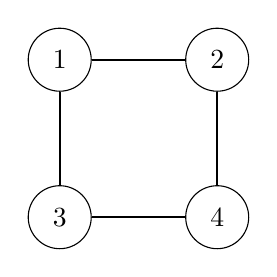
\begin{tikzpicture}[node distance=2cm,
    every node/.style={circle,draw,minimum size=0.8cm}]
    \node (1) {1};
    \node (2) [right of=1] {2};
    \node (3) [below of=1] {3};
    \node (4) [below of=2] {4};
    
    \draw[thick] (1) -- (2);
    \draw[thick] (1) -- (3);
    \draw[thick] (2) -- (4);
    \draw[thick] (3) -- (4);
\end{tikzpicture}
\end{center}

\textbf{Adjacency Matrix}:
\[
\bm{A} = \begin{bmatrix}
0 & 1 & 1 & 0 \\
1 & 0 & 0 & 1 \\
1 & 0 & 0 & 1 \\
0 & 1 & 1 & 0
\end{bmatrix}
\]

This is the $4$-cycle $1 - 2 - 4 - 3 - 1$. Nodes $1$ and $4$ have the same row, and so do nodes $2$ and $3$, so by \cref{graph-autoencoders:rem:identical} the encoder gives $\bm y_1 = \bm y_4$ and $\bm y_2 = \bm y_3$, and the decoder gives them the same reconstructed rows. \textbf{Suppose} the encoder produces
\begin{align*}
\bm{y}_1 = \bm y_4 &= [0.5, 0.5], \qquad
\bm{y}_2 = \bm y_3 = [1.0, 0.5],
\end{align*}
and the decoder reconstructs
\[
\tilde{\bm{A}} = \begin{bmatrix}
0.05 & 0.90 & 0.85 & 0.10 \\
0.90 & 0.05 & 0.10 & 0.92 \\
0.90 & 0.05 & 0.10 & 0.92 \\
0.05 & 0.90 & 0.85 & 0.10
\end{bmatrix}
\]
(the decoder does not know which entry of a row is the diagonal one, so rows $1$ and $4$, and rows $2$ and $3$, are equal).

\subsection*{Computing $\mathcal{L}_{2^{nd}}$ (with $\beta = 5$)}

For node 1: $\bm{A}_1 = [0, 1, 1, 0]$, $\tilde{\bm{A}}_1 = [0.05, 0.90, 0.85, 0.10]$

Weight vector: $\bm{B}_1 = [1, 5, 5, 1]$

Error: $\bm{A}_1 - \tilde{\bm{A}}_1 = [-0.05, 0.10, 0.15, -0.10]$

Weighted error: $[-0.05, 0.50, 0.75, -0.10]$

Squared norm: $0.0025 + 0.25 + 0.5625 + 0.01 = 0.825$

For node 2: $\bm{A}_2 = [1, 0, 0, 1]$, $\bm B_2 = [5, 1, 1, 5]$, error $[0.10, -0.05, -0.10, 0.08]$, weighted error $[0.50, -0.05, -0.10, 0.40]$, squared norm $0.25 + 0.0025 + 0.01 + 0.16 = 0.4225$.

Nodes $4$ and $3$ repeat nodes $1$ and $2$:
\begin{align*}
\mathcal{L}_{2^{nd}}(1) = \mathcal{L}_{2^{nd}}(4) &= 0.825, \qquad
\mathcal{L}_{2^{nd}}(2) = \mathcal{L}_{2^{nd}}(3) = 0.4225 .
\end{align*}
Total: $\mathcal{L}_{2^{nd}} = 2(0.825 + 0.4225) = 2.495$.

\subsection*{Computing $\mathcal{L}_{1^{st}}$}

The graph has edges: $(1,2), (1,3), (2,4), (3,4)$

\begin{align*}
\norm{\bm{y}_1 - \bm{y}_2}^2 = \norm{\bm{y}_1 - \bm{y}_3}^2 = \norm{\bm{y}_2 - \bm{y}_4}^2 = \norm{\bm{y}_3 - \bm{y}_4}^2 = \norm{[-0.5, 0]}^2 = 0.25 .
\end{align*}
Each edge appears twice in the double sum: $\mathcal{L}_{1^{st}} = 2(4\times0.25) = 2.0$.

\subsection*{Computing Total Loss}

With $\alpha = 1$ and $\lambda = 0.001$, and assuming $\norm{\bm{W}}^2_F = 100$:

\begin{align*}
\mathcal{L}_{total} &= \mathcal{L}_{2^{nd}} + \alpha \mathcal{L}_{1^{st}} + \lambda \mathcal{L}_{reg} \\
&= 2.495 + 1 \cdot 2.0 + 0.001 \cdot 100 \\
&= 2.495 + 2.0 + 0.1 \\
&= 4.595
\end{align*}
\end{example}

\section{Training Procedure}

\subsection{Algorithm}

\begin{algorithm}
\caption{Training Graph Autoencoder (SDNE)}
\begin{algorithmic}[1]
\Require Graph adjacency matrix $\bm{A}$, embedding dimension $d$, hyperparameters $\alpha, \beta, \lambda$
\Ensure Node embeddings $\{\bm{y}_i\}_{i=1}^n$
\State Initialize encoder weights $\bm{W}^{enc}$ and decoder weights $\bm{W}^{dec}$
\For{epoch = 1 to $N_{epochs}$}
    \For{batch $\mathcal{B}$ of nodes}
        \State \textbf{Forward pass:}
        \State \quad Encode: $\bm{Y}_{\mathcal{B}} = f_{\bm{W}^{enc}}(\bm{A}_{\mathcal{B}})$ \Comment{Get embeddings}
        \State \quad Decode: $\tilde{\bm{A}}_{\mathcal{B}} = g_{\bm{W}^{dec}}(\bm{Y}_{\mathcal{B}})$ \Comment{Reconstruct adjacency}
        \State
        \State \textbf{Compute losses:}
        \State \quad $\mathcal{L}_{2^{nd}} = \sum_{i \in \mathcal{B}} \norm{(\tilde{\bm{A}}_i - \bm{A}_i) \hadamard \bm{B}_i}^2$
        \State \quad $\mathcal{L}_{1^{st}} = \sum_{i,j \in \mathcal{B}} A_{ij} \norm{\bm{y}_i - \bm{y}_j}^2$
        \State \quad $\mathcal{L}_{reg} = \norm{\bm{W}^{enc}}^2_F + \norm{\bm{W}^{dec}}^2_F$
        \State \quad $\mathcal{L}_{total} = \mathcal{L}_{2^{nd}} + \alpha \mathcal{L}_{1^{st}} + \lambda \mathcal{L}_{reg}$
        \State
        \State \textbf{Backward pass:}
        \State \quad Compute gradients: $\nabla_{\bm{W}^{enc}} \mathcal{L}_{total}$, $\nabla_{\bm{W}^{dec}} \mathcal{L}_{total}$
        \State \quad Update weights using optimizer (e.g., Adam)
    \EndFor
\EndFor
\State \Return Final embeddings $\{\bm{y}_i\}_{i=1}^n$
\end{algorithmic}
\end{algorithm}

\subsection{Computational Complexity}

\begin{itemize}
    \item \textbf{$\mathcal{L}_{2^{nd}}$}: the input and output layers have width $n$, and the loss involves every entry of each reconstructed row, edges and non-edges alike. With a first hidden layer of width $h$, one epoch costs $O(n^2h)$ (sparse inputs reduce the encoder side to $O(\abs Eh)$, but the decoder still produces $n$ outputs per node).
    \item \textbf{$\mathcal{L}_{1^{st}}$}: $O(\abs Ed)$, one term per edge.
\end{itemize}

For large graphs, the input dimension (number of nodes) can be millions, making naive implementations infeasible. Solutions include:
\begin{itemize}
    \item Mini-batch training
    \item Sampling neighborhoods
    \item Using Graph Neural Networks (GNNs) instead
\end{itemize}

\section{Interpretation and Properties}

\subsection{What Does the Embedding Space Learn?}

The trained embeddings have several interesting properties:

\begin{intuition}[Communities and bridges]
Nodes of the same densely connected community share many neighbours, so the reconstruction term places them close, and the first-order term shortens the many edges inside the community. A node with neighbours in two communities is pulled towards both and tends to lie between the two clusters.
\end{intuition}

\subsection{Visualization Example}

We trained SDNE on the karate club graph (\cref{graph-autoencoders:sec:karate_club}) with $d = 2$: encoder $34 \to 16 \to 2$ and decoder $2 \to 16 \to 34$ with $\tanh$ hidden units and sigmoid outputs, $\beta = 5$, $\lambda = 10^{-4}$ on the weight matrices, $\alpha = 1$, Adam with learning rate $0.01$ for $3000$ full-batch steps (PyTorch, seed $0$). \Cref{graph-autoencoders:fig:karate} shows the embeddings coloured by the faction each member joined after the split. To measure the effect of the first-order term we fit a linear classifier (least squares on the two coordinates) and report the fraction of members on the correct side: $53\%$ for $\alpha = 0$, against $94\%$, $91\%$ and $94\%$ for $\alpha = 0.01, 0.1$ and $1$. Without the first-order term the reconstruction is good, but the arrangement of the codes ignores the factions.

\begin{figure}[ht]
\centering
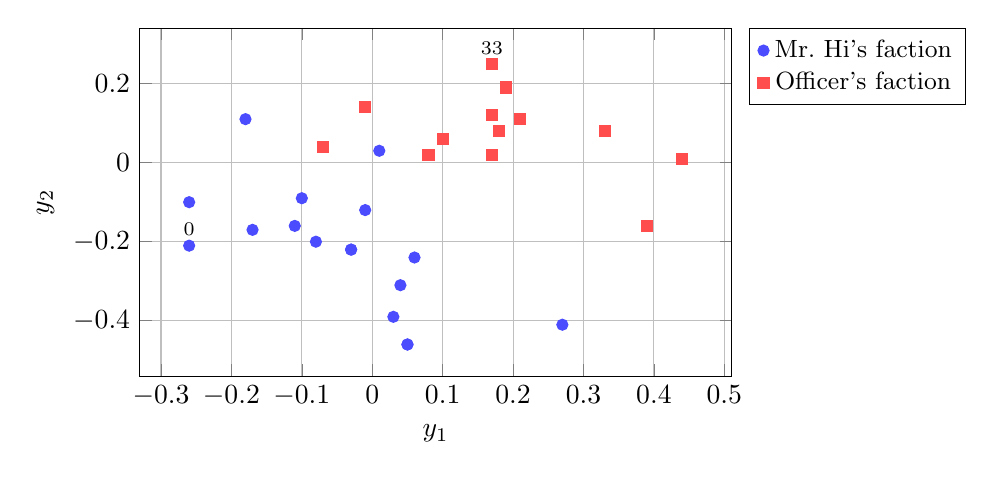
\begin{tikzpicture}
\begin{axis}[width=0.75\linewidth, height=6cm, ymax=0.34, xlabel={$y_1$}, ylabel={$y_2$}, grid=both, legend pos=outer north east, legend style={font=\small}]
\addplot[only marks, mark=*, mark size=2pt, blue!70] coordinates {(-0.26,-0.21) (-0.26,-0.10) (-0.18,0.11) (-0.17,-0.17) (0.04,-0.31) (0.05,-0.46) (0.05,-0.46) (-0.11,-0.16) (0.01,0.03) (0.03,-0.39) (0.06,-0.24) (-0.08,-0.20) (-0.10,-0.09) (0.27,-0.41) (-0.03,-0.22) (-0.01,-0.12) (-0.03,-0.22)};
\addlegendentry{Mr.\ Hi's faction}
\addplot[only marks, mark=square*, mark size=2pt, red!70] coordinates {(0.08,0.02) (0.17,0.02) (0.17,0.02) (0.17,0.02) (0.17,0.02) (0.17,0.02) (0.33,0.08) (0.18,0.08) (0.21,0.11) (0.39,-0.16) (0.17,0.12) (0.10,0.06) (0.44,0.01) (-0.07,0.04) (-0.01,0.14) (0.19,0.19) (0.17,0.25)};
\addlegendentry{Officer's faction}
\node[font=\scriptsize, anchor=south] at (axis cs:-0.26,-0.21) {0};
\node[font=\scriptsize, anchor=south] at (axis cs:0.17,0.25) {33};
\end{axis}
\end{tikzpicture}
\caption{SDNE embedding ($d = 2$, $\alpha = 1$) of Zachary's karate club graph, computed as described in the text. Node $0$ is the instructor, node $33$ the club officer. Two members lie on the wrong side of the best linear separator: node $8$ (Mr.\ Hi's faction) and node $30$ (the officer's). Node $8$, member $9$ in Zachary's numbering, is also the one member that Zachary's minimum cut misassigned.}
\label{graph-autoencoders:fig:karate}
\end{figure}

\section{The Karate Club Graph}
\label{graph-autoencoders:sec:karate_club}

\subsection{Historical Context}

The Zachary's Karate Club graph is one of the most famous datasets in network science. It was collected by anthropologist Wayne Zachary in the 1970s during a study of a university karate club.

\begin{remark}[The story]
Zachary observed social interactions between 34 members of a karate club over a period of 3 years (1970-1972). During this time, a conflict arose between the club's instructor (Mr. Hi) and the club's administrator (John A.) over various issues including the instructor's pricing policies.

This conflict eventually led to a split of the club into two separate organizations. Zachary modelled the network as a flow network and showed that a minimum cut separating the instructor from the officer, computed from ties observed before the split, assigned all but one member to the faction they actually joined (Zachary, \emph{An Information Flow Model for Conflict and Fission in Small Groups}, 1977).
\end{remark}

\subsection{Graph Properties}

\begin{itemize}
    \item \textbf{Nodes}: 34 (club members)
    \item \textbf{Edges}: 78 (social interactions outside of club activities, such as socializing at bars and attending karate tournaments together)
    \item \textbf{Two main communities}: 
    \begin{itemize}
        \item Instructor's faction (loyal to Mr. Hi)
        \item Administrator's faction (loyal to John A.)
    \end{itemize}
    \item \textbf{Bridge nodes}: Members with connections to both factions who faced difficult decisions during the split
\end{itemize}

\subsection{Why It's Important}

The Karate Club graph has become a standard benchmark in network science because:

\begin{enumerate}
    \item \textbf{Real-world validation}: The network structure predicts the actual social split (all members but one, in Zachary's analysis)
    \item \textbf{Clear community structure}: It exhibits two well-defined communities with some inter-community connections
    \item \textbf{Manageable size}: With only 34 nodes, it's small enough to visualize completely and understand intuitively
    \item \textbf{Complex enough}: Despite its size, it demonstrates important phenomena like community detection, bridge nodes, and the predictive power of network analysis
    \item \textbf{Historical significance}: It's one of the earliest examples of using network analysis to understand and predict social phenomena
\end{enumerate}

The Karate Club graph is now a standard benchmark for:
\begin{itemize}
    \item Community detection algorithms
    \item Graph embedding methods
    \item Social network analysis techniques
    \item Network visualization approaches
\end{itemize}

\section{Practical Implementation}

\subsection{Python Implementation Snippet}

The GEM library of Goyal and Ferrara provides an implementation of SDNE (the library targets older versions of Python and TensorFlow; a short PyTorch implementation such as the one used for \cref{graph-autoencoders:fig:karate} is an alternative):

\begin{verbatim}
import networkx as nx
from gem.embedding.sdne import SDNE

# Load Karate Club graph
G = nx.karate_club_graph()

# Initialize SDNE
sdne = SDNE(
    d=2,                # embedding dimension
    beta=5,             # edge weight for reconstruction
    alpha=1e-5,         # first-order loss weight
    nu1=1e-6,           # L1 regularization
    nu2=1e-6,           # L2 regularization
    K=3,                # number of layers
    n_units=[50, 15],   # hidden layer sizes
    rho=0.3,            # corruption level for denoising
    n_iter=10,          # number of iterations
    xeta=0.01,          # learning rate
    n_batch=100         # batch size
)

# Learn embeddings
sdne.learn_embedding(G)
embeddings = sdne.get_embedding()

# embeddings: array of shape (34, 2), one row per node
\end{verbatim}

\subsection{Hyperparameter Tuning}

\begin{table}[h]
\centering
\begin{tabular}{@{}lll@{}}
\toprule
\textbf{Parameter} & \textbf{Typical Range} & \textbf{Effect} \\ \midrule
$\beta$ & 5-10 & Higher = more focus on edge reconstruction \\
$\alpha$ & $10^{-5}$ to $10^{-2}$ & Higher = more first-order preservation \\
$\lambda$ & $10^{-6}$ to $10^{-4}$ & Higher = more regularization \\
$d$ & 2-128 & Embedding dimension \\
layers & 2-4 & Deeper = more expressive (but harder to train) \\ \bottomrule
\end{tabular}
\caption{Typical hyperparameter ranges for SDNE}
\end{table}

\section{Advantages and Limitations}

\subsection{Advantages}

\begin{itemize}
    \item \textbf{Preserves both local and global structure} through combined loss
    \item \textbf{Handles weighted graphs} naturally via $S_{ij}$
    \item \textbf{Non-linear embeddings} capture complex relationships
    \item \textbf{End-to-end differentiable} enables gradient-based optimization
\end{itemize}

\subsection{Limitations}

\begin{itemize}
    \item \textbf{Scalability}: Input dimension equals number of nodes (problematic for large graphs)
    \item \textbf{Transductive}: Cannot directly embed new nodes without retraining
    \item \textbf{No node features}: Only uses graph structure (though can be extended)
    \item \textbf{Hyperparameter sensitivity}: Requires careful tuning of $\alpha$, $\beta$, $\lambda$
\end{itemize}

\subsection{When to Use SDNE}

Use SDNE when:
\begin{itemize}
    \item Graph has $<100,000$ nodes
    \item Need to preserve both community structure and local connections
    \item Have computational resources for training
    \item Don't need to embed new nodes after training
\end{itemize}

Consider alternatives when:
\begin{itemize}
    \item Graph is very large ($>1$ million nodes) $\rightarrow$ use sampling-based methods (DeepWalk, Node2Vec)
    \item Need inductive capability $\rightarrow$ use GNNs (GraphSAGE, GAT)
    \item Have rich node features $\rightarrow$ use feature-aware methods
\end{itemize}

\section{Graph Autoencoders with a GNN Encoder (GAE, VGAE)}

SDNE's encoder reads one adjacency row at a time and has an input layer of width $n$. Kipf and Welling (\emph{Variational Graph Auto-Encoders}, 2016) proposed instead to compute all embeddings at once with a graph convolutional network on node features $X \in \R^{n\times p}$ (or $X = I$ when there are no features) and to decode with inner products.

\begin{definition}[Graph autoencoder (GAE)]
The encoder is a two-layer GCN, $\bm Y = \hat A\,\mathrm{ReLU}(\hat AXW^{(1)})W^{(2)} \in \R^{n\times d}$ with $\hat A = \tilde D^{-1/2}(A + I)\tilde D^{-1/2}$ as in \cref{dft-to-gnn:sec:gcn}. The decoder predicts each edge from the inner product of its endpoints, $\tilde A_{ij} = \sigma(\bm y_i^\top\bm y_j)$, and training minimizes the binary cross-entropy
\[
\mathcal L_{\text{GAE}} = -\sum_{i,j}\Bigl[w\,A_{ij}\log\tilde A_{ij} + (1 - A_{ij})\log(1 - \tilde A_{ij})\Bigr],
\]
where the weight $w$ (the ratio of non-edges to edges) plays the role of SDNE's $\beta$.
\end{definition}

The inner-product decoder has no parameters, so, as for the shallow methods of \cref{ch:shallow-embeddings}, the geometry of the embeddings must itself encode the edges. Because the encoder is a GCN, it uses node features, and it applies to nodes or graphs not seen in training whenever their features and neighbourhoods are known.

\paragraph{Variational graph autoencoder (VGAE).} In the variational version, two GCN heads output for each node a mean $\boldsymbol\mu_i$ and a diagonal log-variance $\log\boldsymbol\sigma_i^2$, the embedding is sampled as $\bm y_i = \boldsymbol\mu_i + \boldsymbol\sigma_i\odot\boldsymbol\varepsilon_i$ with $\boldsymbol\varepsilon_i \sim \mathcal N(0, I)$ (the reparameterization trick), and the loss is the negative evidence lower bound
\[
-\E_q\Bigl[\sum_{i,j}\log p(A_{ij}\mid\bm y_i,\bm y_j)\Bigr] + \sum_i\mathrm{KL}\bigl(\mathcal N(\boldsymbol\mu_i, \diag\boldsymbol\sigma_i^2)\,\|\,\mathcal N(0, I)\bigr),
\]
with the same inner-product likelihood $p(A_{ij} = 1\mid\bm y_i,\bm y_j) = \sigma(\bm y_i^\top\bm y_j)$. Kipf and Welling report that both GAE and VGAE outperform spectral clustering and DeepWalk for link prediction on citation networks, and that node features help substantially.

\paragraph{Other variants.} Attention-based encoders replace the GCN aggregation by learned weights $\bm y_i = \sum_{j\in\mathcal N(i)}\alpha_{ij}\bm h_j$ (graph attention autoencoders, Salehi and Davulcu, 2019). Deep Graph Infomax (Veličković et al., 2019) drops reconstruction altogether and trains the encoder to maximize the mutual information between node embeddings and a summary of the whole graph, with a contrastive objective of the kind studied in \cref{ch:contrastive-learning}.

\begin{chaptersummary}
\begin{itemize}
\item A plain reconstruction loss on adjacency rows is dominated by the zeros of a sparse graph. SDNE weights the errors on edges by $\beta > 1$ inside the norm, $\mathcal L_{2^{nd}} = \sum_i\norm{(\tilde{\bm A}_i - \bm A_i)\odot\bm B_i}^2$, which preserves second-order proximity.
\item The first-order term $\mathcal L_{1^{st}} = \sum_{i,j}S_{ij}\norm{\bm y_i - \bm y_j}^2 = 2\tr(\bm Y^\top L\bm Y)$ shortens edges; alone it is minimized by collapsing all embeddings, so the two terms are complementary.
\item An encoder that reads adjacency rows maps structurally equivalent nodes (identical rows) to the same embedding, whatever the loss; distinguishing them requires features or identities in the input.
\item GAE and VGAE encode with a GCN and decode with $\sigma(\bm y_i^\top\bm y_j)$; VGAE adds a Gaussian posterior per node and a KL term. They use node features and scale better than SDNE, whose input width is $n$.
\end{itemize}
\end{chaptersummary}

\section*{Further reading}
\addcontentsline{toc}{section}{Further reading}
SDNE is due to Wang, Cui and Zhu (\emph{Structural Deep Network Embedding}, 2016), and GAE and VGAE to Kipf and Welling (\emph{Variational Graph Auto-Encoders}, 2016). Hamilton (\emph{Graph Representation Learning}, 2020, Chapters~3 and~6) places them in the encoder--decoder view of node embeddings. The karate club data come from Zachary (1977).

\section*{Exercises}
\addcontentsline{toc}{section}{Exercises}

\begin{exercise}\label{graph-autoencoders:exr:1}
A graph has $n$ nodes and average degree $\bar d$; each row $\bm A_i$ has $n$ entries (the diagonal one is $0$). Compute the unweighted reconstruction loss $\sum_i\norm{\tilde{\bm A}_i - \bm A_i}^2$ of the model that outputs $\tilde{\bm A} = 0$, and of the model that outputs the constant $c = \bar d/n$ everywhere. With the SDNE weights, for which $\beta$ does the constant output $\frac12$ have a smaller loss than the zero output?
\solutionlink{graph-autoencoders:exr:1}
\end{exercise}

\begin{exercise}\label{graph-autoencoders:exr:2}
Prove \cref{graph-autoencoders:eq:l1_trace} for a symmetric weight matrix $S$, and deduce that the minimizers of $\mathcal L_{1^{st}}$ on a connected graph are exactly the configurations with all $\bm y_i$ equal.
\solutionlink{graph-autoencoders:exr:2}
\end{exercise}

\begin{exercise}\label{graph-autoencoders:exr:3}
Minimize $\mathcal L_{1^{st}}$ for the path $1 - 2 - 3$ with $d = 1$ under the constraints $\bm Y^\top D\bm Y = 1$ and $\bm Y^\top D\mathbf 1 = 0$ (Laplacian eigenmaps). Where do nodes $1$ and $3$ end up, and why does this not contradict \cref{graph-autoencoders:rem:identical}?
\hint{Generalized eigenproblem $L\bm y = \mu D\bm y$.}
\solutionlink{graph-autoencoders:exr:3}
\end{exercise}

\begin{exercise}\label{graph-autoencoders:exr:4}
For VGAE with $d$-dimensional embeddings, compute in closed form the divergence
\[
\mathrm{KL}\bigl(\mathcal N(\boldsymbol\mu, \diag\boldsymbol\sigma^2)\,\|\,\mathcal N(0, I)\bigr),
\] and its value for $\boldsymbol\mu = (1, 0)$, $\boldsymbol\sigma = (1, \frac12)$.
\solutionlink{graph-autoencoders:exr:4}
\end{exercise}

\end{notechapter}
